\section{The solution: OCULAR}

In this thesis a software has been developed that is intended to be used in assistive and social robots.
The name and the logo (figure \ref{ocular_logo}) of the project gives a first idea of the system's goal. 
The name of the project, OCULAR, is an acronym of "On-line objeCt Learning And Recognition". 
The first word, on-line, refers to the fact that the learning of new objects is done in real time. % there is no need of a training phase in which the software is not operative. 
Figure \ref{ocular_logo} presents the logo of the software, which gives two additional pieces of information: 
The object learning and recognition is performed in-hand and the input of the system an RGB-D sensor, such as a Kinect. 
This type of sensor provides 2D and 3D information of the user located in front of it. 

\\

\begin{figure}[H]
	\begin{center}
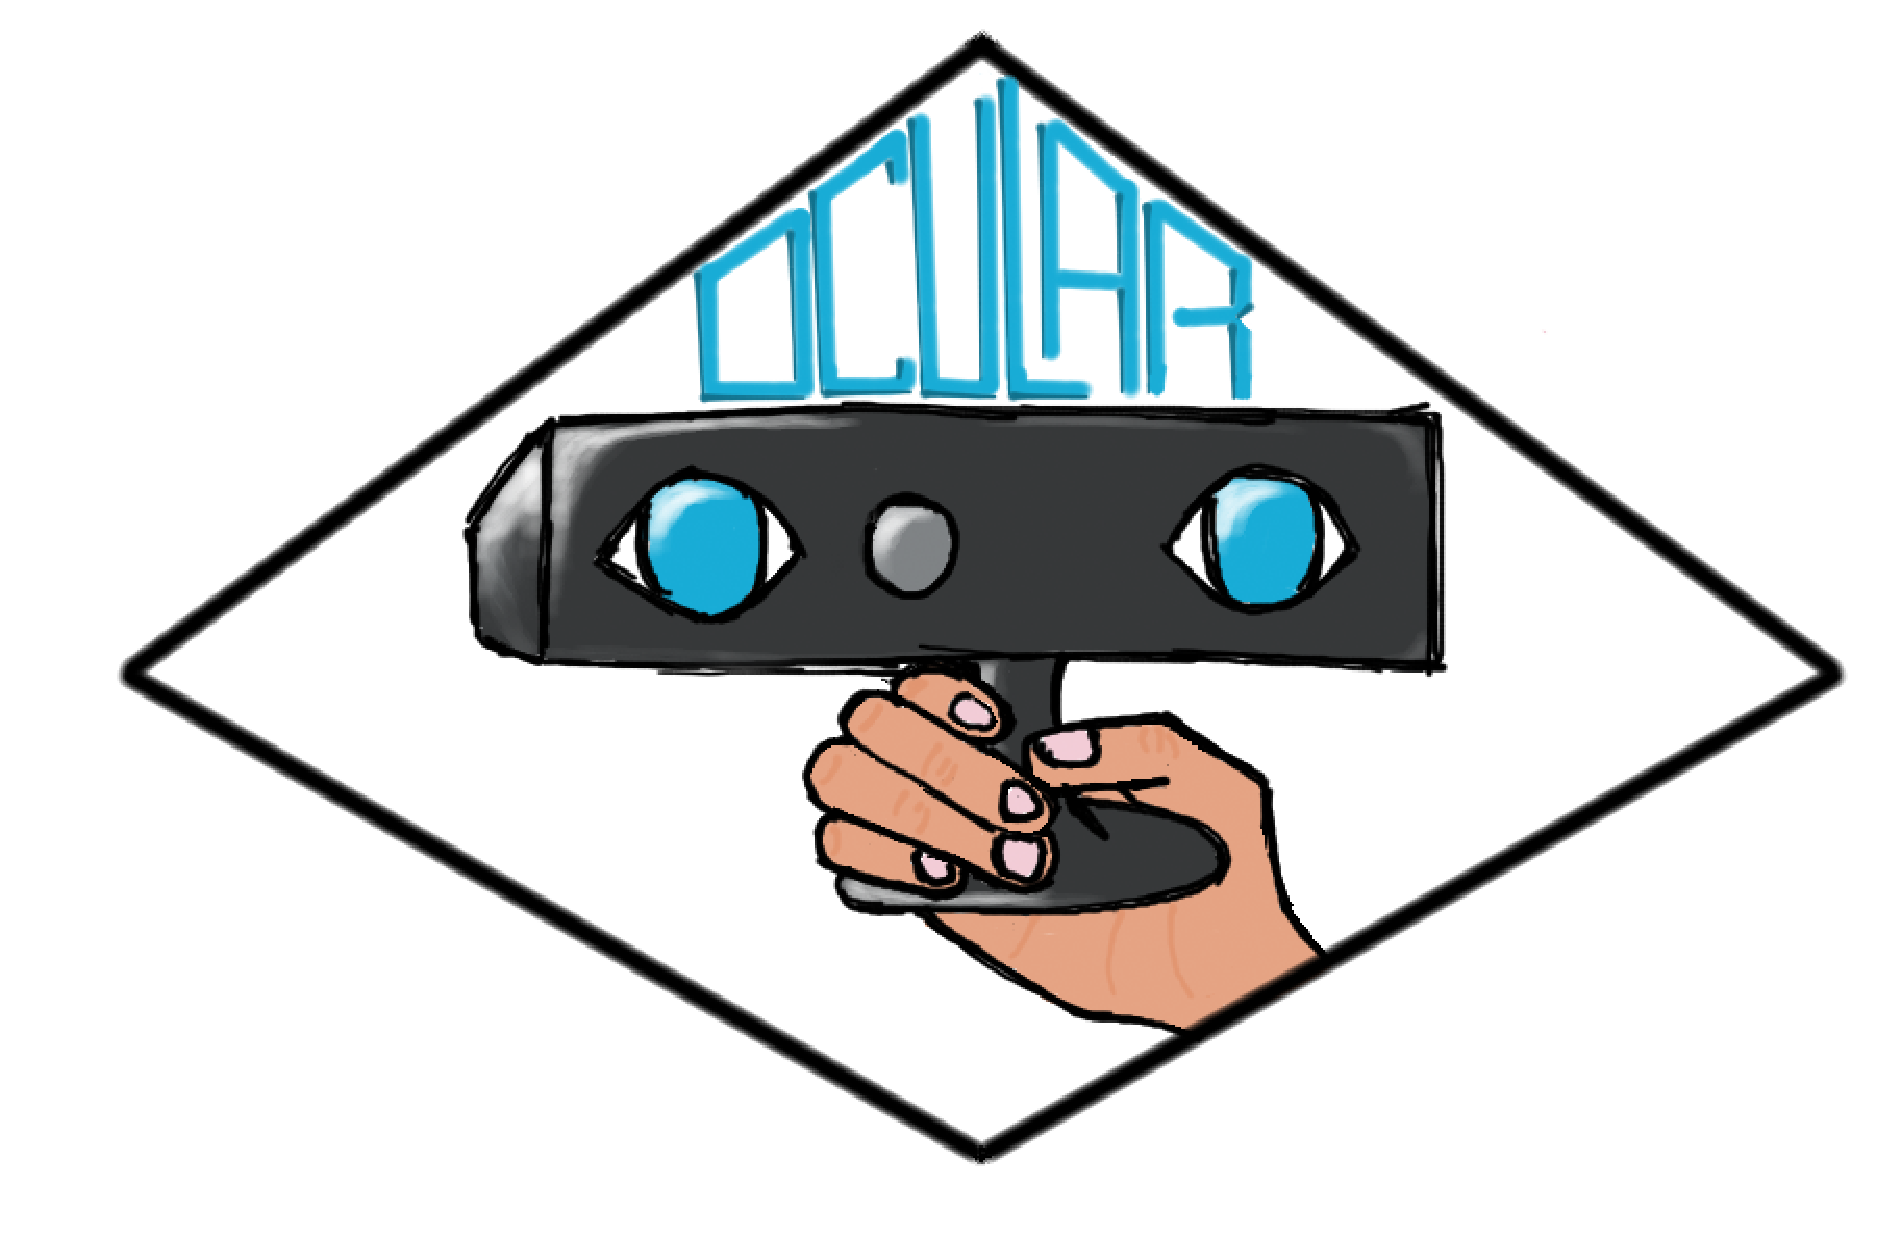
\includegraphics[scale=0.3]{img/ocular_logo.eps}
	\caption[OCULAR Logo]{OCULAR logo}
		\label{ocular_logo}
	\end{center}
\end{figure}

Since it is intended to be running on a robot, the software has to implement an intuitive human-machine interface. 
A gestural interface was designed that allows the passing of information from human to computer in a simple way. 
The software has two differentiated modes, the learning or data acquisition mode and the recognition or system exploitation modes. 
The system is able to detect the change of the mode using the pose of the user as can be seen in figures \ref{learn} and \ref{recognize}. 
% The usability of the software is fully dependent on the easy transition for the user from one mode to the other. 
% Furthermore, the humans can hold an object with either hand and the information of which hand is holding the object must be passed to the program. 
% The gesture was designed to have the most comfortable and easy to maintain posture possible. 
In order to trigger the learning mode, the user only needs to extend his arm towards the sensor, showing the item to it (figure \ref{learn}. 
This is a natural gesture usually performed between humans when introducing new objects to one another. 
Having the hand closer to the body the recognition mode is triggered and the program outputs a unique id for the learned object (figure \ref{recognize}). 

% \vspace*{0.5cm}



	
\begin{figure}[H]
   \centering
   \begin{subfigure}[H]{0.45\textwidth}
       \centering
		\includegraphics[width=\textwidth]{img/intro/learn.png}
		\caption[Learning Mode Triggering]{\textbf{Learning mode} triggering using the gestural interface. The learning phase starts when the user stretches the arm towards the RGB-D sensor. The system takes a definable number of views of each object, with a delay between views of 1 second. This allows the user to change the object's pose. }    	 
		\label{learn}
   \end{subfigure}
   \hfill
   \begin{subfigure}[H]{0.45\textwidth}
       \centering
    	\includegraphics[width=\textwidth]{img/intro/recognize.png}
		\caption[Recognizing Mode Triggering]{\textbf{Recognizing mode} triggering using the gestural interface. When the user pulls his hand closer to the body and the learning phase has finished, the recognizing mode starts. It is the default mode of the software. This means that if no event occurs the system keeps outputting the unique ID for the learned object that was recognized. }      
		\label{recognize}

   \end{subfigure}
   \caption{OCULAR working modes}
   \label{}
\end{figure}






% \begin{figure}[H]
% 	\centering
%     \includegraphics[width=0.5\textwidth]{img/intro/learn.png}
% 	\caption[Learning Mode Triggering]{Learning mode triggering using the gestural interface. The learning phase starts when the user stretches the arm towards the RGB-D sensor. The system takes a definable number of views of each object, with a delay between views of 1 second. This allows the user to change the object's pose. }
% 	\label{learn}
% \end{figure}
% \vspace*{0.5cm} 
%  % The software is able to work with one hand at a time, and the hand that is located the highest is the one being used. 

% \vspace*{0.5cm}
% \begin{figure}[H]
% 	\centering
%     \includegraphics[width=0.5\textwidth]{img/intro/recognize.png}
% 	\caption[Recognizing Mode Triggering]{Recognizing mode triggering using the gestural interface. When the user pulls his hand closer to the body and the learning phase has finished, the recognizing mode starts. It is the default mode of the software. This means that if no event occurs the system keeps outputting the unique ID for the learned object that was recognized. }
% 	\label{recognize}
% \end{figure}

% \vspace*{0.5cm}

Apart from switching modes evaluating the user's pose, the system also detects the hand that is holding an object. 
The software is able to work with one hand at a time and it chooses the one that is higher. 

The present project has been designed to be as modular and reusable as possible making an easier task to develop complementary software such as handbags recognition or hats recognition with slightly modifications. Its structure consists on nodes that run on parallel and minimizes the lag due to the computing processes. It is an Open Source project, meaning that anyone can use and modify it.
\\

In order to facilitate the usage of the code it has been developed as a ROS \cite{ros} package. The source code and further installation instructions and license details might be found in the following link to the software's \href{http://github.com/irenesanznieto/ocular}{\color{blue}\underline {repository}}. 
